% !TEX root =../LibroTipoETSI.tex
\chapter{Pruebas realizadas}\LABCHAP{EntornoPrueba}
\pagestyle{esitscCD}

\epigraph{What gets measured, gets managed.}{Peter Drucker}

\lettrine[lraise=-0.1, lines=2, loversize=0.25]{E}n este capítulo presentamos las pruebas realizadas al software con el 
fin de validar su comportamiento.

Se comenzará con las pruebas de laboratorio en la \SEC{PruebasLaboratorio}, destacando las más importantes para 
verificar el correcto funcionamiento de la aplicación, especialmente en el tema de falsos positivos 
(\SSEC{FalsosPositivos} y falsos negativos (\SSEC{FalsosNegativos}.

Para concluir, se pasará a una prueba más real y relevante realizada en Produban en la sección \SEC{PruebaProduban}

%TODO falta mas datos

\section{Pruebas de laboratorio}\LABSEC{PruebasLaboratorio}
\subsection{Entorno del laboratorio}

\begin{figure}[htbp]
\centering
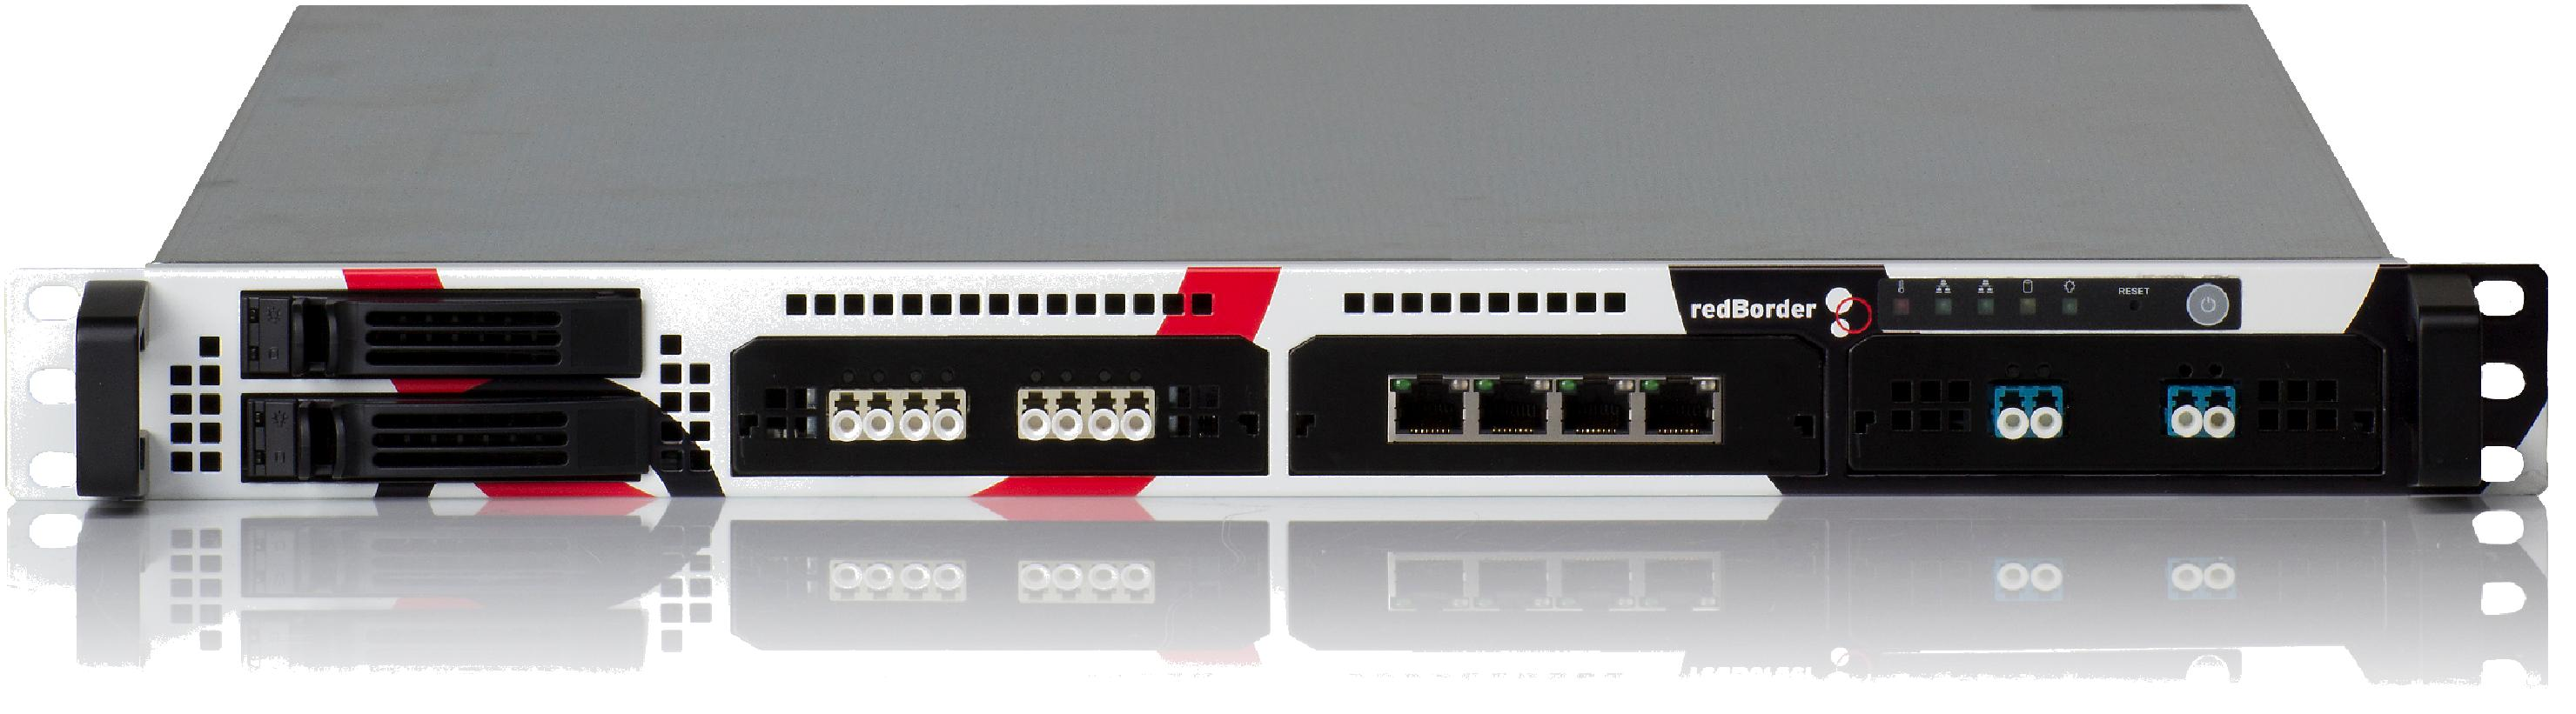
\includegraphics[width=\textwidth]{CapituloPruebas/Figuras/Sensor}
\caption{Device Under Test}
\LABFIG{DUT}
\end{figure}
%

El equipo \gls{DUT} es un redBorder IPS de 8 hilos (1 quad-core de 2 hilos por core) Intel Xeon E3-1240 a 3.30GHz. La 
interfaz del segmento de inspección es una intel quad-ethernet 82580 Gigabit con soporte bypass. En el sensor se ha 
instalado la distribución \emph{redBorder-IPS-sensor 3.0.30-1}, basada en la distribución Linux CentOS 6.5.

Como generador de tráfico, se usará otro dispositivo con las mismas características. Los segmentos de $1G$ se unirán de 
un equipo a otro en el mismo orden, a fin de facilitar el entendimiento de las pruebas, y serán llamados 
\text{eth4}, \text{eth5}, \text{eth6}, y \text{eth7} de izquierda a derecha.

En estos momentos, el controlador actual de la tarjeta de $10G$ no soporta $ZeroCopy$, por lo que habrá que hacer las 
pruebas en $1G$.

Se dispone, además de una captura de tráfico llamada \emph{entrenamiento.pcap}, que contiene tráfico real sin ataques.

\subsection{Prueba 1: Ajuste de los parámetros CUSUM para evitar falsos positivos}\LABSSEC{FalsosPositivos}
\subsubsection{Descripción de la prueba}
El primer paso de cara a realizar las pruebas es conseguir un valor adecuado de los parámetros $k$ y $h$. Como vimos en 
\CHAP{Algoritmo CUSUM}, el parámetro $k$ indica la magnitud que debe tener una muestra $x_i$ para que sume algo a 
$C_{i-1}$, en unidades de $\left[\sigma\right]$. El parámetro $h$, por su parte, indica el número de desviaciones 
típicas que debe alcanzar $C_i$ para que se deba lanzar una alerta.

Recordamos en \EQ{PruebasCusumPos} y \EQ{PruebasCusumNeg} las ecuaciones del algoritmo \gls{CUSUM}, por comodidad.
\begin{align}
 K &:= k\sigma \nonumber\\
 H &:= h\sigma \nonumber\\
 C_i^+ &= C_{i-1}^+ + (x_i-\mu_0-K) \LABEQ{PruebasCusumPos} \\
 C_i^+ &= C_{i-1}^+ - (x_i-\mu_0-K) \LABEQ{PruebasCusumNeg} \\
 &\text{Alarma si $C_i^\cdot > H$} \nonumber
\end{align}

\subsubsection{Procedimiento}
En procedimiento de la prueba será el siguiente:
\begin{enumerate}
 \item Se debe conocer la duración de la captura. 
 \item Se arranca el programa con un periodo de entrenamiento ligeramente inferior, ya que si la captura termina antes 
de tiempo, se registrarán muestras $0$ lo cual disminuirá la media. Por otro lado, si se repitiese, también disminuiría 
la desviación típica, lo que tampoco nos conviene.
 \item Tras el periodo de entrenamiento, se debe crear un fichero en \texttt{/var/log/ddos.log.<timestamp>} con los 
estadísticos registrados en ese periodo de tiempo.
 \item Se debe hacer pasar de nuevo la capruta por el sensor, pre-cargando los estadísticos con el parámetro 
\texttt{-l}, y con unos valores iniciales de $k$ y $h$. Se deben modificar a fin de encontrar unos valores que no 
generen alertas, ya que son claramente falsos positivos.
 \begin{enumerate}
  \item Si, tras un tiempo, existen varias direcciones \gls{IP} con un valor $C_i$ demasiado elevado, es porque $k$ 
estaba muy bajo.
  \item Si existen muchas alertas con valores $C_i$ bajos, es porque $h$ es demasiado bajo.
 \end{enumerate}
\end{enumerate}

Para lanzar la captura, se usó el comando tcpreplay, tras generar el archivo .cache:

\begin{verbatim}
[ @trafficgen pcap]$ tcpprep -i entrenamiento.pcap -o entrenamiento.cache
[ @trafficgen pcap]$ tcpreplay --cachefile entrenamiento.cache --intf1=eth4 --intf2=eth5
\end{verbatim}

Por su parte, \redborderddos fue lanzado con los siguientes parámetros en el entrenamiento:

\begin{verbatim}
[root@DUT rbddos]# ./rbddos -i eth4 -o eth7 -c 99 -r 0 -g 1:2:3:4:5:6  -m 7 -d -s 1024
\end{verbatim}

Y de esta otra manera en el periodo de defensa

\begin{verbatim}
[root@DUT rbddos]# ./rbddos -i eth4 -o eth7 -c 99 -r 0 -g 1:2:3:4:5:6  -m 7 -d -s 1024 -l /var/log/ddos.log.*
\end{verbatim}

Donde los parámetros usados significan:

\begin{verbatim}
 -i    Interfaz de entrada
 -o    Interfaz de salida
 -c    PF_RING cluster id
 -r    Núcleo usado para el balanceador
 -g    Núcleos usados para los contadores
 -m    Núcleo usado por el contador principal
 -d    Modo depuración
 -s    Tamaño de la piscina de contadores
 -l    Archivo de datos aprendidos
\end{verbatim}

Como valores iniciales, se escogieron los recomendados por Ismael Sánchez, $k=2.5$ y $h=5$ \cite{CUSUM_Carlos_III}.

\subsubsection{Resultados}
Tras realizar las pruebas, se observó que los valores negativos $C_i^-$ eran muy propensos a anunciar alarmas, deido 
a que el tráfico suele ser la mayor parte del tiempo $0$ y, durante un breve intervalo de tiempo, elevado. Por lo 
tanto, los distintos flujos están demasiado tiempo inactivos, lo que hace que se lance su alarma asociada.

% TODO
% Paquetes: 00, 01, 02, 03, 04, 05, 06, 07, 08, 09
% Total: 1528795 150000 ...
% ICMP: 15330 6614 5488 3651 5795 9547 4497 4939 4060 5440

Debido también a demasiadas alarmas, aquellas relacionadas con el protocolo \gls{ICMP} también tuvieron que ser 
desactivadas. La traza contenía muy pocos paquetes de este protocolo ($65361$ de $15000000$), por lo que se decidió 
descartar estas alarmas.

Finalmente, los parámetros para evitar falsas alarmas fueron ajustados a $k=5$ y $h=10$.

\subsection{Prueba 2: Detección de IPs atacantes, control de falsos negativos y estado de 
alerta}\LABSSEC{FalsosNegativos}
\subsubsection{Descripción de la prueba}
Para esta prueba, se necesitarán las cuatro interfaces de red. Con el aprendizaje de la prueba anterior, se hará pasar 
la captura \emph{entrenamiento.pcap} por uno de los dos segmentos, mientras que en el otro, al cabo de un tiempo $T_0$, 
se hará pasar tráfico claramente atacante: una ráfaga de paquetes UDP a alta velocidad, desde un pcap preparado.

Se modificará \texttt{rbddos} para que emita un mensaje si, en un ciclo, se ha visto bajo ataque, y para que emita el 
tráfico total visto. De esta forma, podremos saber si el programa funciona correctamente.

Se utilizarán los datos de entrenamiento de la anterior prueba.

\subsubsection{Procedimiento}
Se arranca el programa, ya en modo defensa por los datos aprendidos
\begin{verbatim}
[root@DUT rbddos]# ./rbddos -i eth4 -o eth7 -c 99 -r 0 -g 1:2:3:4:5:6  -m 7 -d -s 1024 -l /var/log/ddos.log.*
\end{verbatim}

Se hace pasar el tráfico por un segmento vía \texttt{tcpreplay}:
\begin{verbatim}
 tcpreplay --cachefile entrenamiento.cache --intf1=eth4 --intf2=eth5 entrenamiento.pcap
\end{verbatim}

Pasados 20 segundos, se hace pasar el tráfico UDP a alta velocidad por el otro segmento:
\begin{verbatim}
 tcpreplay -t --cachefile udp.cache --intf1=eth6 --intf2=eth7 udp.pcap
\end{verbatim}

Se detiene el pcap a los 10 segundos. Tras ello, se analiza la salida, y se registra, con la salida de depuración:
\begin{itemize}
 \item Número de paquetes analizados por el programa.
 \item Si el programa ha estado en alerta o no.
\end{itemize}

\subsubsection{Reultados}

\section{Prueba realizada en Produban}\LABSEC{PruebaProduban}
\subsection{Entorno}
El día 4 de mayo de 2013, Produbán, empresa de gestión IT del grupo Santanter, pidió a Eneo un sistema que de detección 
de ataques \gls{DDoS}, dado que tenía la sospecha de que se iba a producir un ataque real a su infraestructura.

Pese a estar aún en un estado muy prematuro, Produban aceptó la instalación del software ya que no entrañaba riesgo 
para la infraestructura al estar este situado en un puerto SPAN.

\begin{figure}[hbtp]
\centering
%\hfill
\subfloat[Frontal del sensor]%
   {\LABFIG{ProdubanFrontal}%
   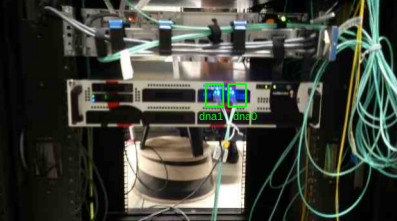
\includegraphics[width=0.49\textwidth]{CapituloPruebas/Figuras/ProdubanFrontal}}
\hfill
\subfloat[Parte trasera del sensor]%
   {\LABFIG{ProdubanTrasera}%
   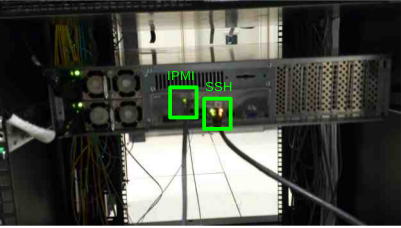
\includegraphics[width=0.49\textwidth]{CapituloPruebas/Figuras/ProdubanTrasera}}
%
\caption{Instalación de \redborderddos{} en el CPD de Mesena, Produban}
\end{figure}
%
El sensor usado es un equipo 2U con doble procesador Xeon E5 y 64GB de RAM, con 2 puertos dedicados de gestión y otros 
2 puertos 10G para conectarse a un puerto de SPAN, y es instalado en el CPD de Mesena.

En la \FIG{ProdubanFrontal} podemos ver la parte frontal del sensor, en la que fueron instalados dos pares de fibra 
óptica dirigidas a un puerto SPAN. Por otro lado, en la parte trasera, vemos la conexión de la interfaz de gestión y el 
puerto IPMI, una interfaz especial dirigida a manejar el sensor por web.

\subsection{Resultados}
Debido a lo inmediato de la instalación, fue imposible ajustar el sensor para que diese resultados significativos. Con 
sólo tres horas de entrenamiento, y sin ser estas siquiera determinantes, era muy difícil que la prueba diese 
resultados satisfactorios.

Los resultados fueron, en cuanto al periodo de aprendizaje:
\begin{table}[htbp]
 \centering
 \begin {tabular}{lll}
  Parámetro & Media & Desviación típica  \\\hline
  Paquetes TCP & 93\% & 0.02 \\
  Paquetes UDP & 5\%  & 0.02 \\
  Paquetes ICMP & 0 & 0      \\
  Relación I/O & 32,41 & 13,75 \\
  Longitud media del flujo & 593.54 & 59.57 \\
  Relación SYN/(SYN+ACK) & 593.54 & 59.57   
 \end {tabular}
\end{table}

Debido al estado altamente prematuro de la aplicación, el resultado de la relación SYN/(SYN+ACK) fue confiundido con el 
de la longitud media del flujo. Esto, junto con el escaso margen que tenían los valores ICMP, provocaron que el número 
de alarmas emitidas fuese enorme.

El programa estuvo ejecutándose desde el 7 de mayo a las 11:53\footnote{Timestamp: 1367920409} hasta el 15 de mayo a 
las 11:36, y se generaron más de 100 millones de alarmas.

Las conclusiones principales que se extrayeron fue que la realidad era mucho más cambiante de lo que permitía discernir 
tres horas de entrenamiento, o incluso un día, y que se debería de adaptar el protocolo CUSUM para hacer frente a esa 
realidad.

\section{Conclusiones}
Tras analizar las pruebas realizadas en este capítulo, se observa que el algoritmo CUSUM se enfrenta bien a las pruebas 
de laboratiorio, pero es incapaz, como lo hemos planteado, de hacer frente a una muestra variable como es el tráfico 
que enfrenta un sistema a lo largo del tiempo. Así pues, se deberán buscar o bien otros sistemas de control de 
procesos, o bien modificar el algoritmo CUSUM para lograr analizar correctamente dicha variablidad.


\endinput

